\section{OpenMax}

\begin{frame}{softmax}
\centering
	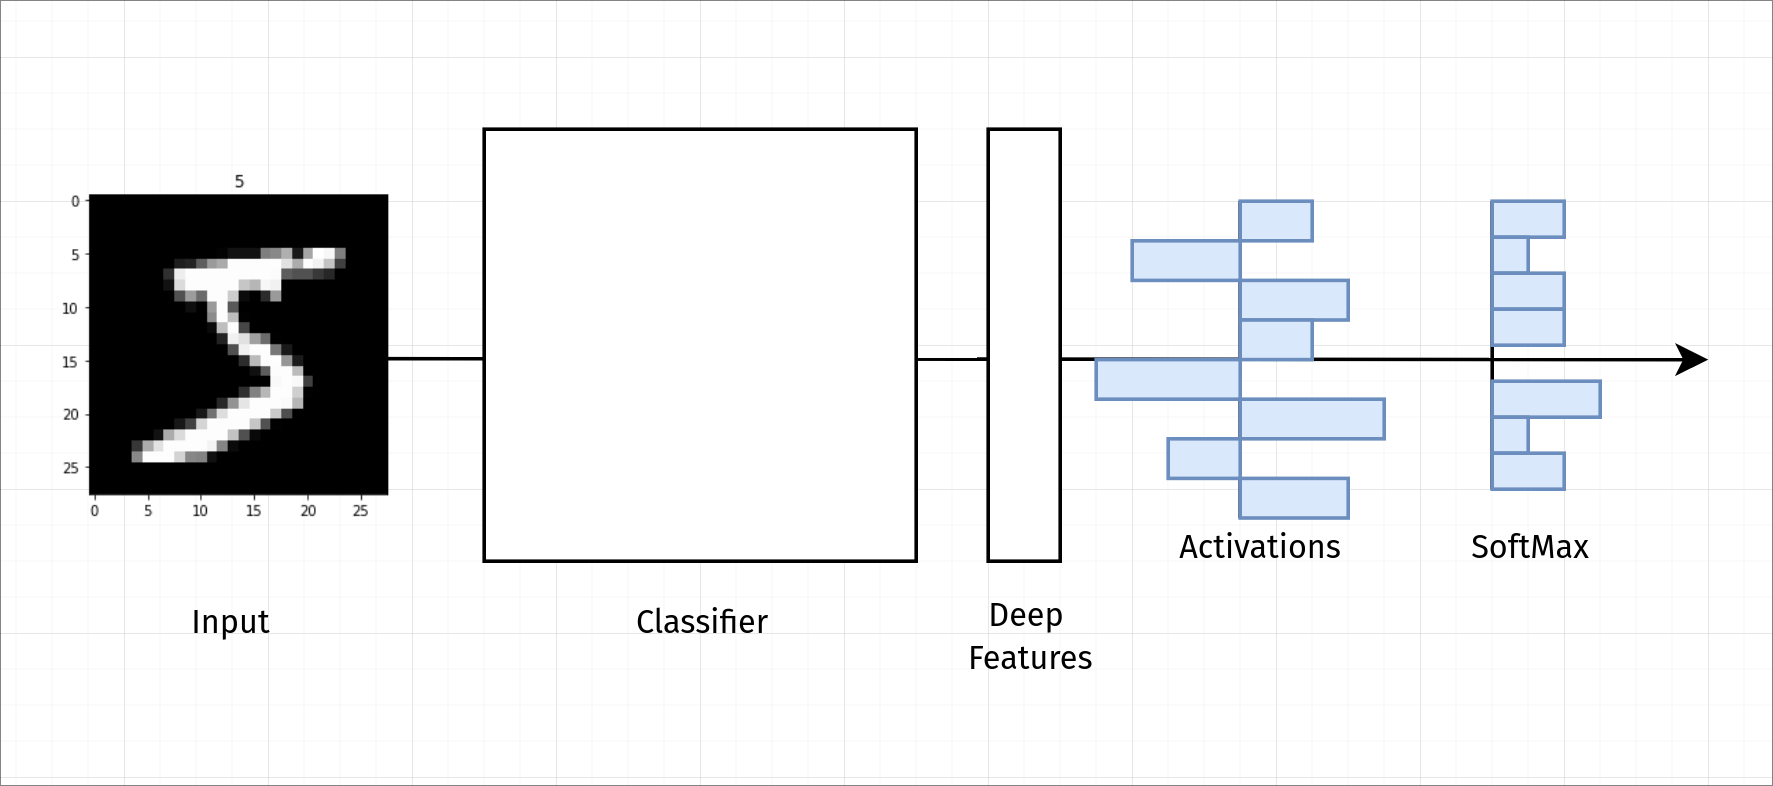
\includegraphics[width=\textwidth]{figures/softmax.png}
\end{frame}

\begin{frame}{Introducing OpenMax}
	\begin{itemize}
		\item Extension of SoftMax during testing
		\item Distance based
		\item Deep features
		\item Extreme Value Theory
		\item Heuristic
	\end{itemize}
\end{frame}

\begin{frame}{OpenMax Overview}
	\centering
	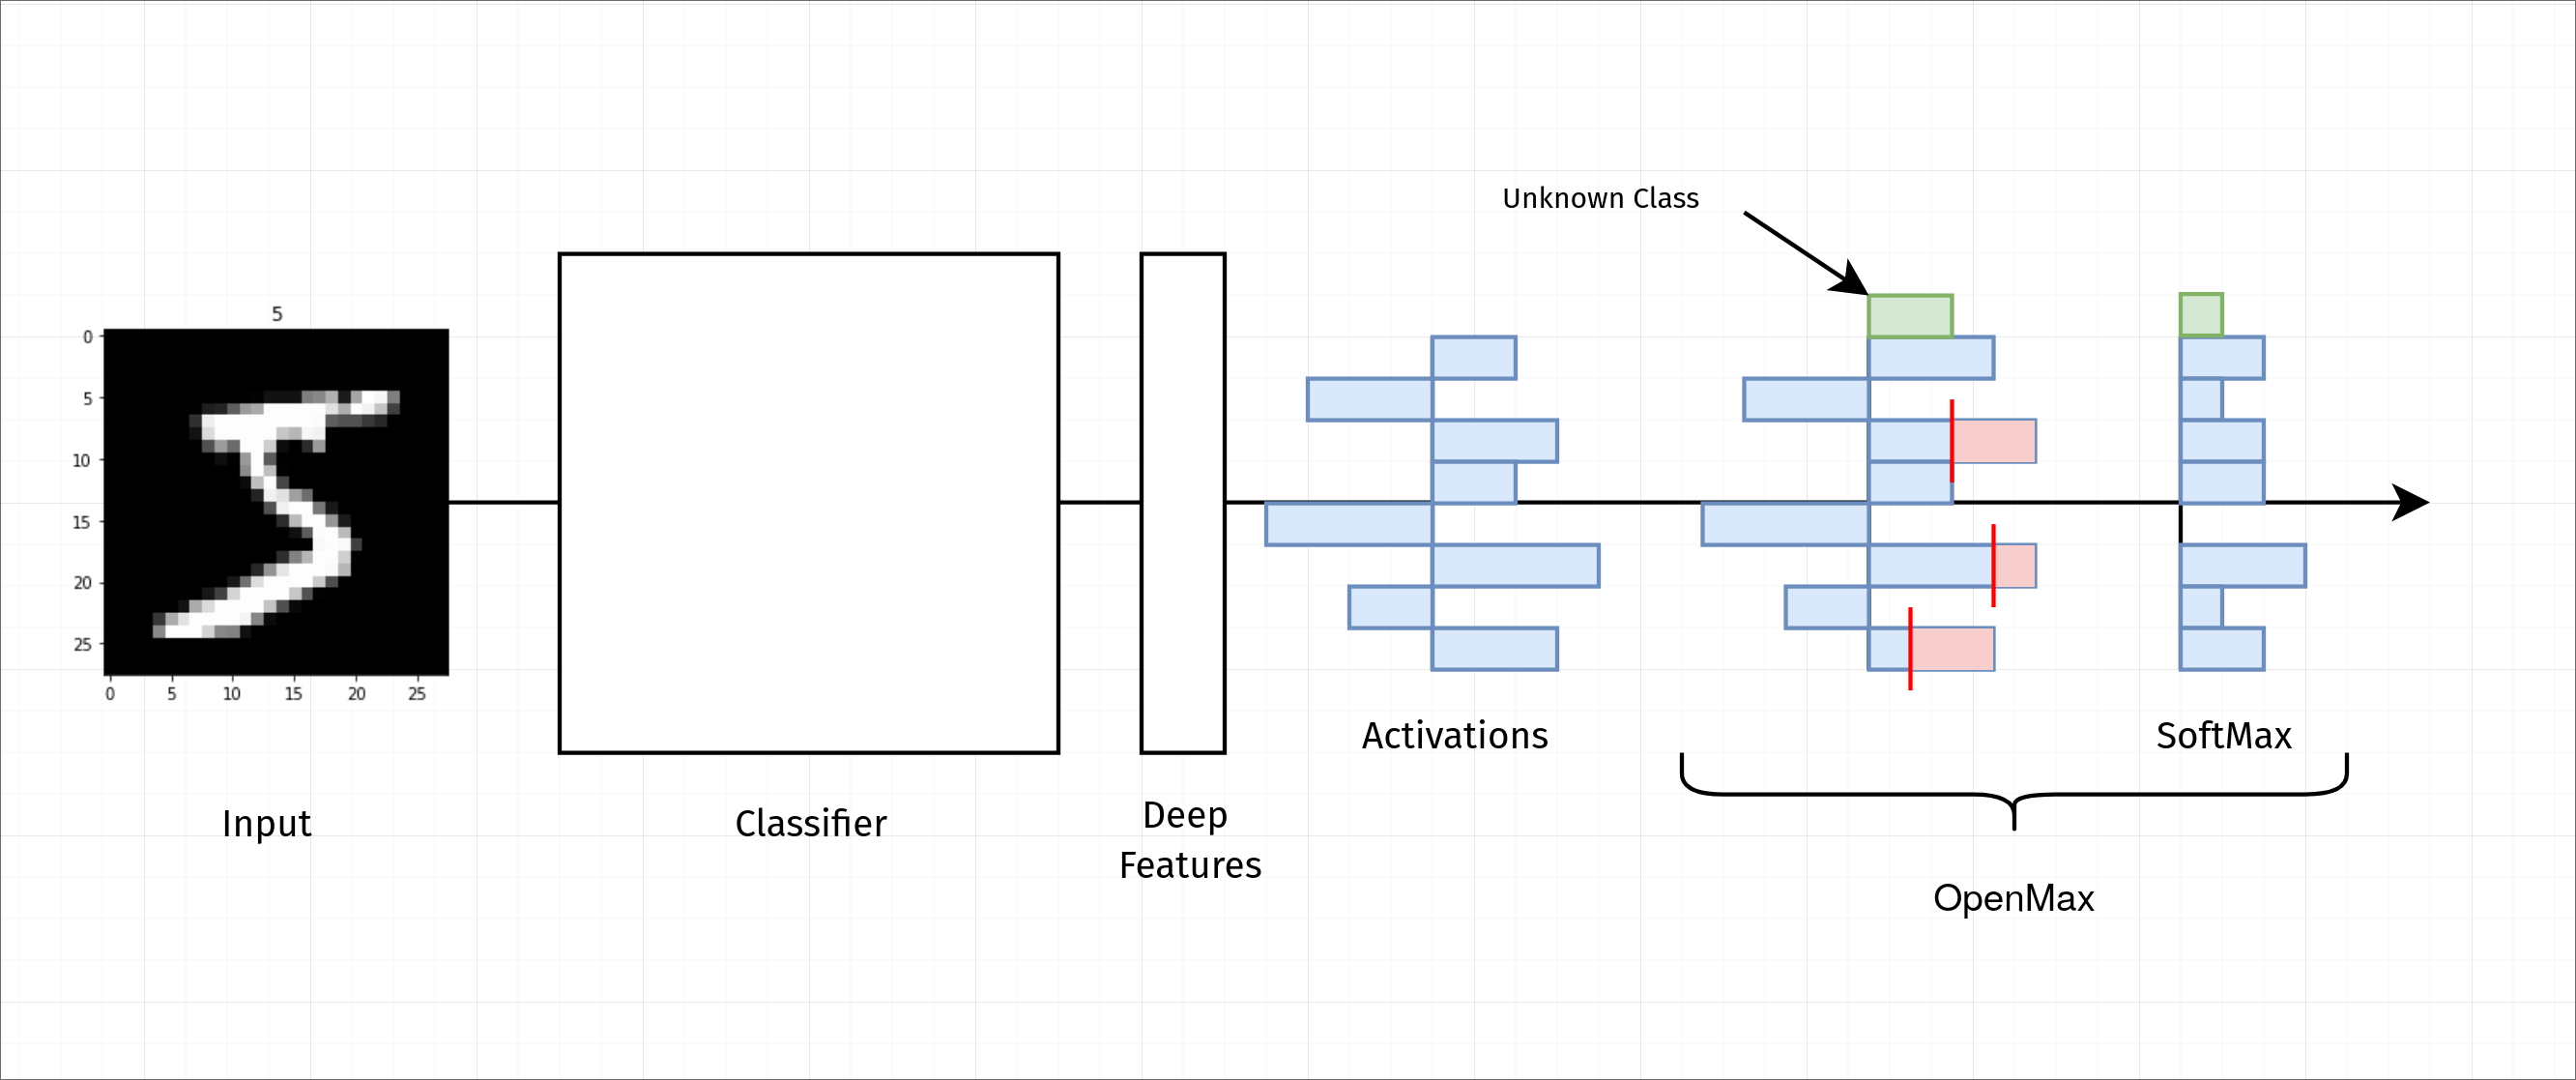
\includegraphics[width=\textwidth]{figures/openmax.drawio.png}
\end{frame}


\begin{frame}{Calibrating OpenMax}
	\begin{itemize}
		\item Training
		\item Class representation
		\item Mean Activation Vector $\mu$
		\item Features from penultimate layer $\phi$
		\item Correctly classified samples
		\item Weibull Distribution
		\item Tail size $\eta$ \& Distance Multiplier $\kappa$
	\end{itemize}
\end{frame}

% \begin{frame}{Weibull Distribution}
% 	\begin{itemize}
% 		\item Confidence Score
% 		\item Models extreme events
% 		\item Distribution tails
% 		\item Point of Failure
% 	\end{itemize}
% \end{frame}

\begin{frame}{Building a Weibull Distribution}
	\centering
	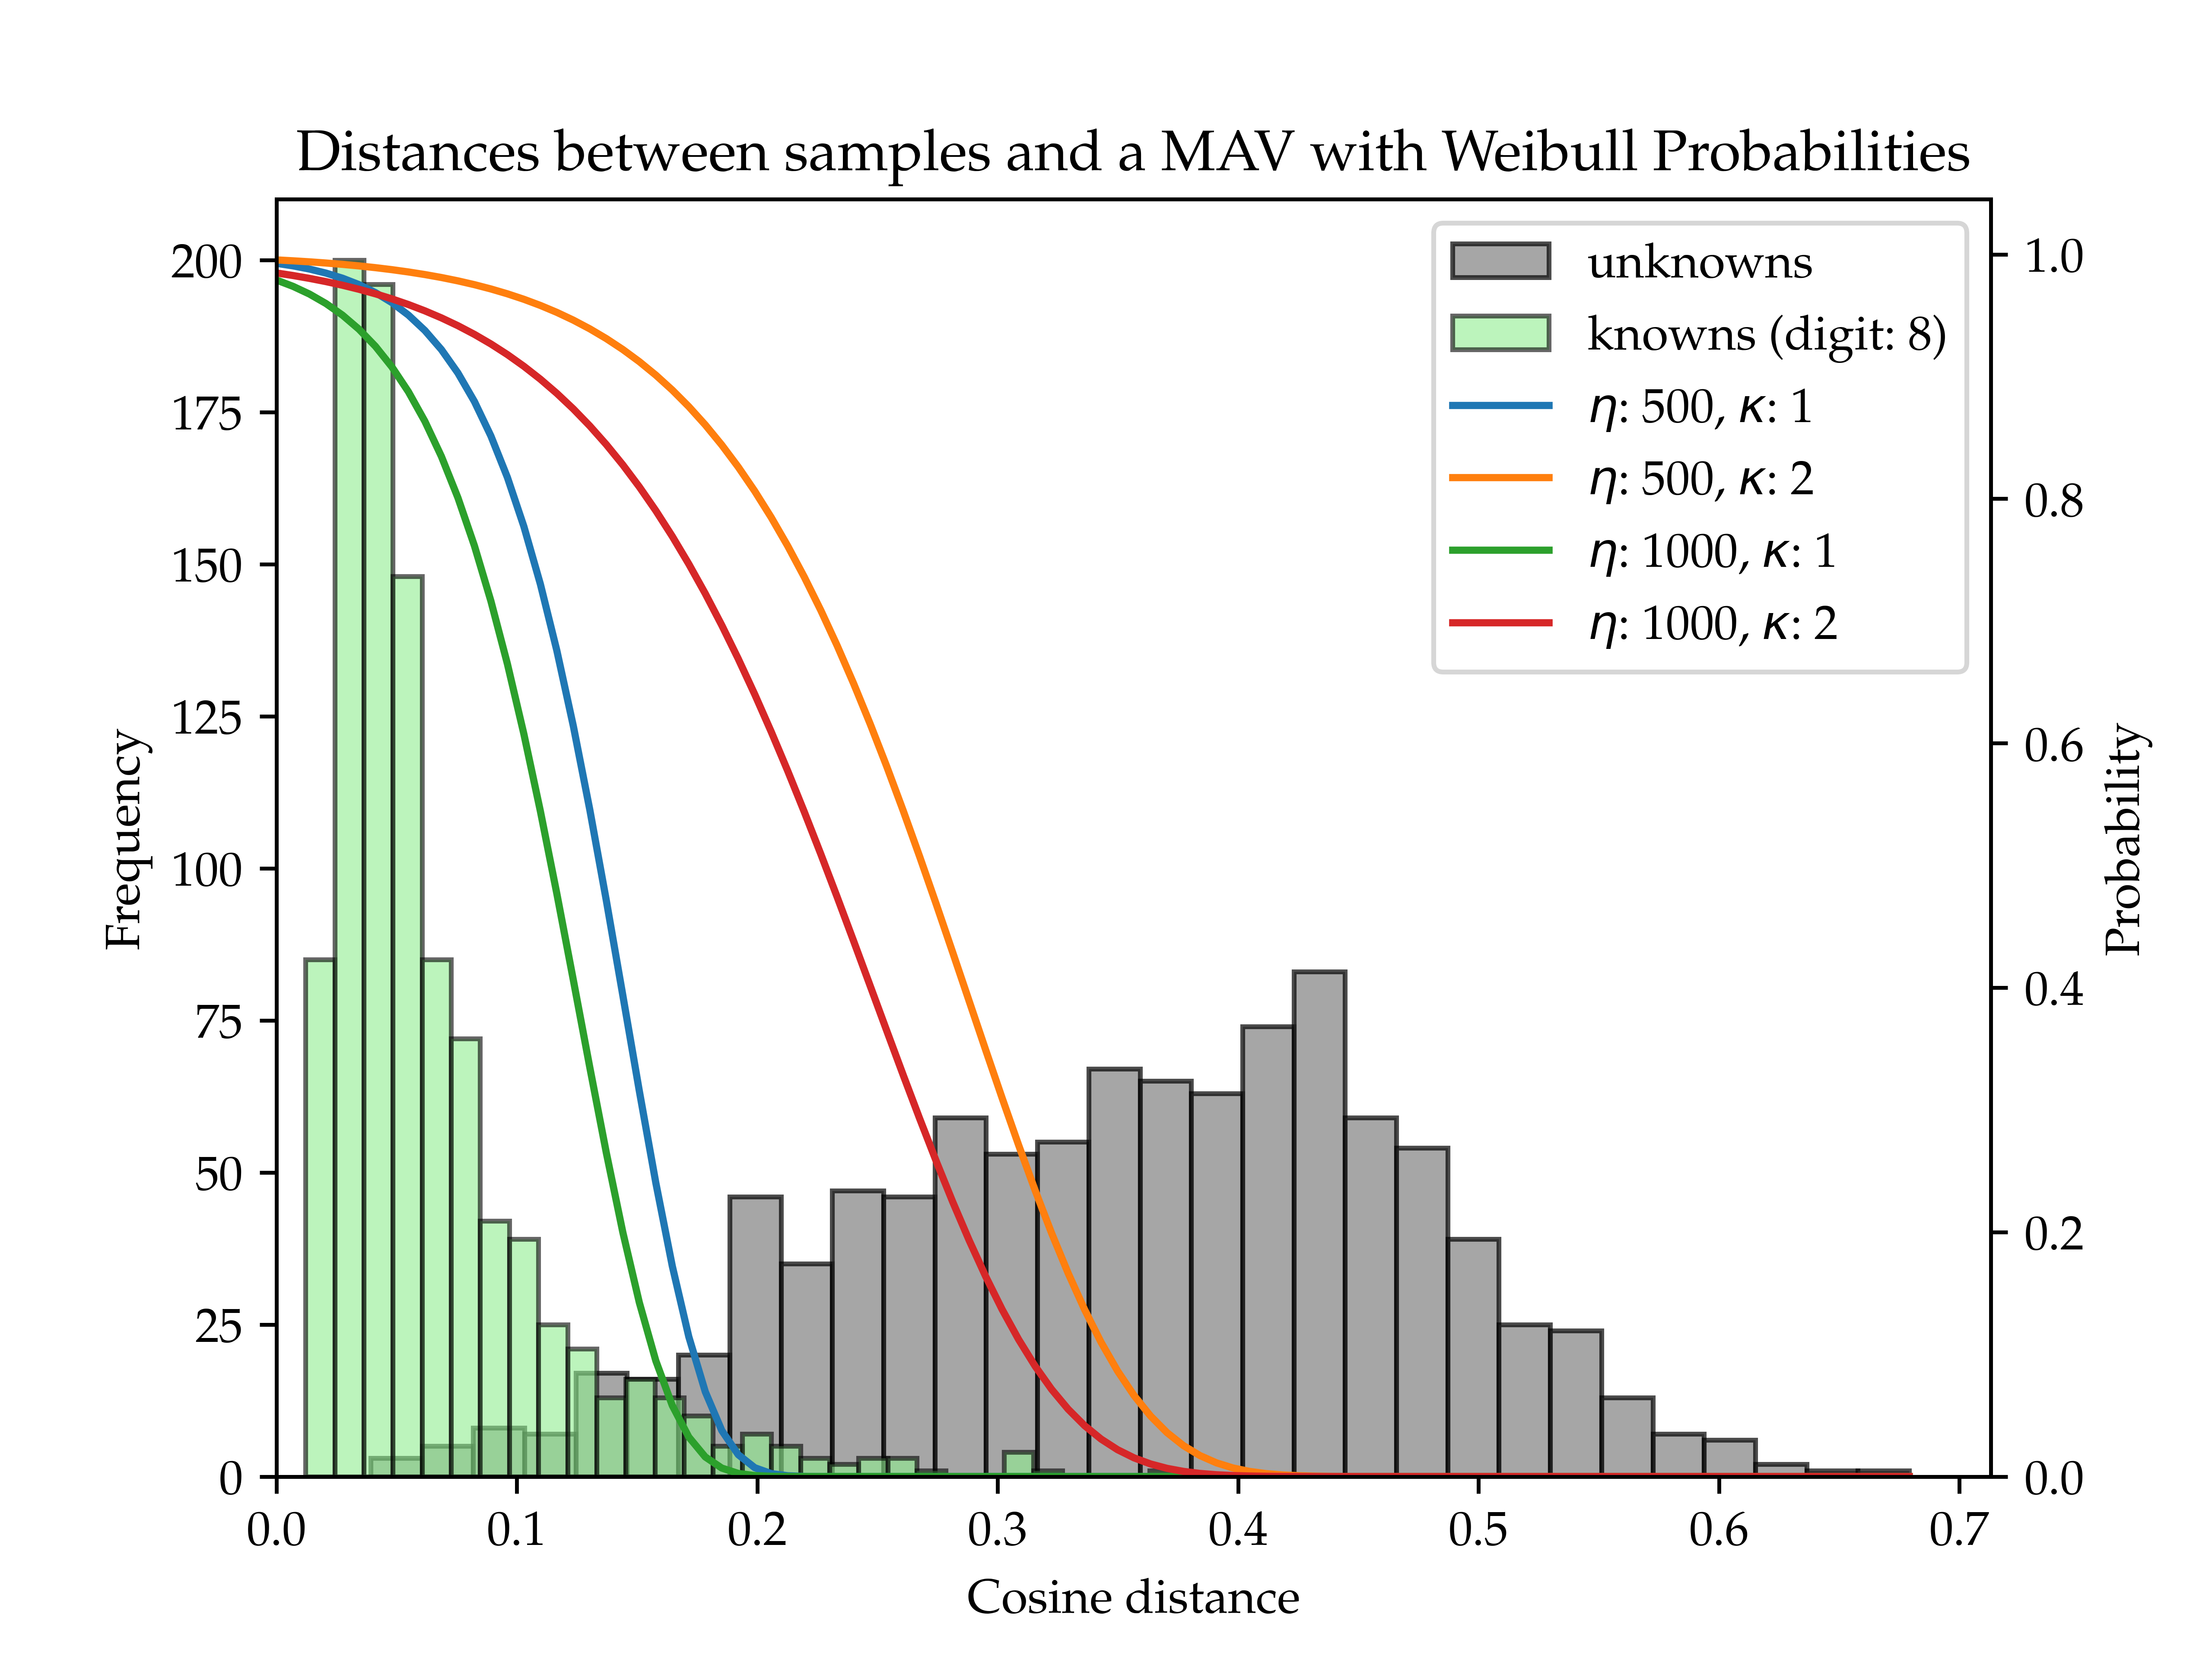
\includegraphics[width=\textwidth]{figures/distances-to-mav.png}
\end{frame}

\begin{frame}{OpenMax in Detail}
	For a testing sample:
	\begin{enumerate}
		\item Sort and select $\alpha$ classes (logit value)
		\item Weibull Probability $\omega$ based on distance $\mu_i$ and $\phi$
		\item $\hat{z} = z \circ \omega $
		\item $\hat{z}_{N+1} = \sum_i z_i (1 - \omega_i)$
		\item $\operatorname{softmax}(\hat{z})$
	\end{enumerate}
\end{frame}


